\section*{Tema 2}
\addcontentsline{toc}{section}{Tema 2}
    Para comenzar definiremos qué no es \textit{testing}:
    \begin{itemize}
        \item No es algo que encuentra todos los defectos
        \item No es presionar todos los botones al azar, esperando que algo falle.
        \item No es simplemente que algo falle
        \item No es algo que puedes hacer después de que se complete toda la programación
        \item No es algo que se pueda posponer hasta que los usuarios comienzan a quejarse
    \end{itemize}
    
    Pero entonces qué sí es el testing, como lo entenderemos en este curso: “En un alto nivel, las pruebas de software son una forma de proporcionar una estimación de la calidad del software a las partes interesadas (es decir, personas que tienen un interés directo en el sistema, como clientes, usuarios y gerentes).”
    
    Una definición alternativa que podemos utilizar: "Es una estrategia de gestión de riesgo en software" 
    
    \subsection*{Requisitos y la importancia para el testing}     
    \addcontentsline{toc}{subsection}{Requisitos y la importancia del testing}
    
        \subsubsection*{Negocio}
        \addcontentsline{toc}{subsubsection}{Negocio}
        
        Es muy común que el equipo de desarrollo pase muy poco tiempo entendiendo el problema real del negocio, las necesidades de los usuarios y otros stakeholders y la naturaleza del entorno en el que sus aplicaciones deben prosperar. Los desarrolladores tendemos a seguir adelante, brindando soluciones tecnológicas basadas en una  \textit{comprensión inadecuada del problema a resolver}.
        
        Preguntas útiles para establecer los requerimientos del negocio, el analista siempre debe preguntar por qué:
        
        \begin{itemize}
            \item ¿Cuál es el problema del negocio que estás tratando de resolver?
            \item ¿Cuál es la motivación para solucionar este problema?
            \item ¿Qué haría por ti una solución exitosa?
            \item ¿Hay algún otro proyecto o sistema que podría influenciar el proyecto o al que este proyecto podría afectar?
            \item ¿Cuáles son los grupos o individuos que podrían influenciar este proyecto o ser influenciados por el?
            \item ¿Podría pensar en alguna consecuencia adversa o inesperada que el nuevo sistema podría causar?
            \item ¿Qué actividades de negocio y eventos deberían ser incluidos en la solución? ¿Cuáles no?
            \item ¿Cuál es el valor de una solución de éxito?
        \end{itemize}
        
        Los requerimientos de negocio sirven para establecer una visión de producto y el alcance del proyecto.
        
        \begin{enumerate}
            \item Requerimientos de negocio
                \begin{itemize}
                    \item Background
                    \item Oportunidad de negocio
                    \item Objetivos de negocio y criterios de éxito
                    \item Necesidades de cliente y mercado
                    \item Riesgos de negocio
                \end{itemize}
            \item Visión de la solución
                \begin{itemize}
                    \item Declaración de visión
                    \item Características principales
                    \item Supuestos y dependencias
                \end{itemize}
            \item Alcance y limitaciones
                \begin{itemize}
                    \item Alcance del \textit{release} inicial
                    \item Alcance de subsecuentes \textit{releases}
                    \item Limitaciones y exclusiones
                \end{itemize}
            \item Contexto del negocio
                \begin{itemize}
                    \item Perfiles de Stakeholders
                    \item Prioridades del proyecto
                    \item Ambiente operativo
                \end{itemize}
        \end{enumerate}
        
        \subsubsection*{Usuarios}
        \addcontentsline{toc}{subsubsection}{Usuarios}
        
            Para establecer los requerimientos de usuario, debemos conocer al usuario real, a quien realmente trabajará con el sistema. En vez de preguntar \textit{¿Qué desea?} o \textit{¿Qué quiere que haga el sistema?}, es mejor usar el enfoque basado en uso y objetivos: \textit{¿Qué necesita hacer con el sistema?}\\
            
            Algunas preguntas útiles para establecer estos requerimientos son:
            
            \begin{multicols}{2}
                \begin{itemize}
                    \item ¿Cuáles son las razones por las que tú o tus colegas usarían el nuevo producto?
                    \item ¿Qué problemas esperas que te resuelva este producto?
                    \item ¿Alguna(s) porción(es) del producto son mas críticas que otras para el rendimiento, confiabilidad, seguridad, disponibilidad u otra característica?
                    \item ¿Cuán  similar es el producto que tú imaginas con la forma como haces tu trabajo actualmente? ¿Cuán diferente debería ser?
                    \item ¿Qué objetivos piensas que este producto te ayudaría a cumplir?
                    \item ¿Qué palabras usarías para describir el producto?
                    \item ¿Hay alguna restricción o regla que el producto deba cumplir?
                    \item ¿Qué aspectos del producto actual o del proceso del negocio deseas retener? ¿Cuáles desearías reemplazar?
                    \item ¿Qué aspectos del producto son más críticos para crear valor al negocio?
                    \item ¿Qué aspectos del producto te entusiasman más?
                    \item ¿Qué es lo más importante del producto para ti?
                    \item ¿Hay algo más que debería preguntar?
                    \item ¿Qué aspectos del producto serán de más valor para ti? ¿Cuáles de menos valor?
                    \item ¿Cómo juzgarías si el producto es un éxito?
                    \item ¿Podrías describir el ambiente en el cual el producto será usado?
                    \item ¿Podrías describir el ambiente en el cual el producto será usado?
                    \item ¿Alguien alguna vez querrá *inserte acción*?
                    \item ¿Alguna vez podrá ocurrir *inserte escenario*?
                    \item ¿Qué pasaría si *inserte condición de error* ocurre?
                \end{itemize}
            \end{multicols}
            
            \newpage
            
        \subsubsection*{Casos de uso}
        \addcontentsline{toc}{subsubsection}{Casos de uso}
        
        Un caso de uso es una secuencia de interacciones entre un sistema y un actor. Los casos de uso son documentos de texto, no diagramas. El modelarlos es una ayuda para escribir el documento, más la finalidad no es dibujar un diagrama. Estos sirven para describir \textit{textualmente} todas las tareas que los usuarios necesitarán ejecutar con el sistema.
        
        Ejemplo de caso de uso:
        
        \begin{table}[h]
\begin{tabular}{|l|l|}
\hline
ID \& name: &
  UC-4 Request a Chemical \\ \hline
Created by: Lori &
  Date created: 22/8/13 \\ \hline
Primary Actor: Requester &
  Secondary actors: Buyer, Chemical Stockroom, Training Database \\ \hline
Description: &
  \begin{tabular}[c]{@{}l@{}}The Requester specifies the desired chemical to request by entering its name or \\ chemical ID number or by importing its structure from a chemical drawing tool. \\ The system either offers the Requester a container of the chemical stockroom or \\ lets the Requester order one from a vendor.\end{tabular} \\ \hline
Trigger: &
  Requester indicates that they want to request a chemical \\ \hline
Preconditions: &
  \begin{tabular}[c]{@{}l@{}}PRE-1: User's identity has been authenticated.\\ PRE-2: User is authorized to request chemicals.\\ PRE-3:Chemical inventory database is online\end{tabular} \\ \hline
Postcontidions: &
  \begin{tabular}[c]{@{}l@{}}POST-1: Request is stored in the CTS.\\ POST-2: Request was sent to the Chemical Stockroom or to a Buyer.\end{tabular} \\ \hline
Normal Flow: &
  \begin{tabular}[c]{@{}l@{}} \textbf{4.0 Request a Chemical from the Chemical Stockroom}\\ 1. Requester specifies the desired chemical.\\ 2. System lists containers of the desired chemical that are in the chemical \\     stockroom, if any.\\ 3. System gives Requester the option to View Container History for any container.\\ 4. Requester selects a specific to ask to place a vendor order (see 4.1).\\ 5. Requester enters other information to complete the request.\\ 6. System stores the request and notifies the Chemical stockroom.\end{tabular} \\ \hline
Alternative Flows: &
  \begin{tabular}[c]{@{}l@{}}\textbf{4.1 Request a Chemical from a Vendor}\\ 1. Requester searches vendor catalogs for the chemical (see 4.1.E1)\\ 2. System displays a list of vendors for the chemical with available container sizes, \\     grades and prices.\\ 3. Requester selects a vendor, container size, grade and number of containers.\\ 4. Requester enter other information to complete the request.\\ 5. System stores the request and notifies the Buyer.\end{tabular} \\ \hline
Exceptions: &
  \begin{tabular}[c]{@{}l@{}}\textbf{4.1.E1 Chemical is not commercially available}\\ 1. System display message: No vendors for that chemical.\\ 2. System ask Requester if they want to rquest another chemical (3a) or exit (4a).\\ 3a. Requester ask to request another chemical.\\ 3b. System starts normal flow over.\\ 4a. Requester ask to exit.\\ 4b. System terminates use case.\end{tabular} \\ \hline
Priority: &
  High \\ \hline
Frecuency of use: &
  \begin{tabular}[c]{@{}l@{}}Approximately 5 times per week by each chemist, 200 times per week by \\ chemical stockroom staff.\end{tabular} \\ \hline
Business rules: &
  BR-28, BR-31 \\ \hline
Other information: &
  \begin{tabular}[c]{@{}l@{}}The system must be able to import a chemical structure in the standar \\ encoded form from any of the supported drawing packages.\end{tabular} \\ \hline
Assumptions: &
  Imported chemical structures are assumed to be valid. \\ \hline
\end{tabular}
\end{table}
        
        \newpage
        \textbf{Recomendaciones para redactar bien los pasos de un caso de uso:}
        
    \begin{enumerate}
        \item Utilizar gramática simple (\textbf{sujeto} + \textit{verbo} + predicado):
        
        \textbf{El sistema} \textit{suma el dinero depositado} en la cuenta del cliente.
        
        \item Debe mostrar claramente \textit{Who has the ball?}
        
        El sistema, ¿qué actor?
        
        \item Muestra que el proceso se mueve claramente hacia adelante.
        \item Está escrito desde el punto de vista de un tercero
        
            Antes:
            \begin{itemize}
                \item "Ingresar nombre de columna"
                \item "Mostrar lista de comercios ubicados en la comuna"
            \end{itemize}
            Después:
            \begin{itemize}
                \item "El usuario ingresa el nombre de la columna"
                \item "El sistema muestra los comercios ubicados en la comuna"
            \end{itemize}
            
        \item Muestra la intención del actor, no sus movimientos:
        
        Antes:
        
        \begin{itemize}
            \item El sistema solicita nombre de usuario
            \item El usuario ingresa su nombre
            \item El sistema solicita dirección del usuario
            \item El usuario ingresa su dirección
            \item El usuario hace click en "OK"
            \item El sistema muestra los datos del usuario
        \end{itemize}
        
        Después:
        
        \begin{itemize}
            \item El usuario ingresa su nombre y dirección
            \item El sistema muestra los datos del usuario
        \end{itemize}
        
        \item No "comprueba si...", simplemente valida:
        
        Antes:
        \begin{itemize}
            \item El sistema valida si la password es correcta
            \item Si la password es correcta, el sistema muestra los porcentajes de descuentos
        \end{itemize}
        
        después
        \begin{itemize}
            \item El sistema valida que la password sea correcta
            \item El sistema muestra los porcentajes de descuentos
        \end{itemize}
        
        \item "Repetir pasos $X-Y$ hasta <condición>"
        
        \begin{enumerate}
            \item[(1)] El sistema muestra lista de productos
            \item[(2)] El usuario marca el producto que desea comprar
            \item[(3)] El sistema añade el producto al carrito de compras del cliente
            
            \begin{itemize}
                \item El cliente repite los pasos (2) - (3) hasta que indique que su compra está lista
            \end{itemize}
            
            \item[(4)] El sistema muestra opciones de pago
            
        \end{enumerate}
        
    \end{enumerate}
    \newpage 
    Ejemplos de diagramas de caso de uso:
    
    \begin{figure}[h]
        \begin{multicols}{2}
            \centering
            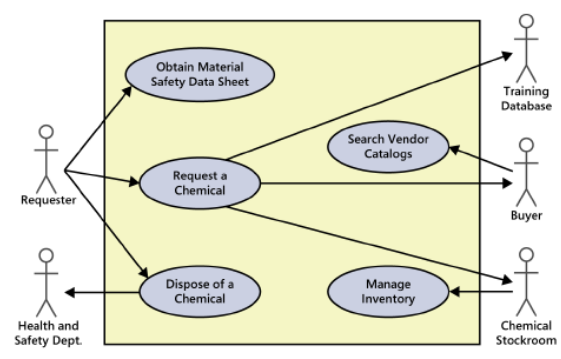
\includegraphics[width=0.42\textwidth]{imgs/7.png}
            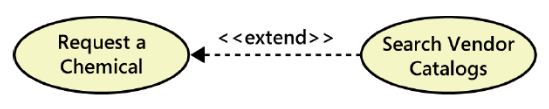
\includegraphics[width=0.4\textwidth]{imgs/8.png}
            
            \vspace{7mm}
            
            Existen situaciones en las que el Caso de Uso de extensión no es indispensable que ocurra, cuando lo hace, ofrece un valor extra al objetivo original del caso uso base.
        \end{multicols}
    \end{figure}
    
    \subsection*{Elicitación, análisis, especificación y gestión de requerimientos}
    \addcontentsline{toc}{subsection}{Elicitación, análisis, especificación y gestión de requerimientos}
    
    El proceso de desarrollo de requerimientos es incremental e iterativo. Pero debido a la diversidad de proyectos de desarrollo y culturas de las organizaciones, no existe una única forma de desarrollar requisitos.
    
    \subsubsection*{Especificación}
    \addcontentsline{toc}{subsubsection}{Especificación}
    
    \textbf{Reglas de negocio}
    
     Cada organización opera de acuerdo con un amplio conjunto de políticas, leyes y estándares de la industria. Las industrias, como la banca, la aviación y la fabricación de dispositivos médicos, deben cumplir con los volúmenes de las regulaciones gubernamentales. Dichos principios de control se conocen colectivamente como reglas o lógica de negocio.
     
     Utilizando una perspectiva empresarial, "una regla de negocio es una \textbf{guía} de que existe una \textbf{obligación} con respecto a la conducta, acción o práctica dentro de una actividad o esfera en particular". Existe una motivación explícita para la regla y métodos de aplicación, existe una comprensión de las consecuencias a ocurrir de romper la regla. Mientras que con la perspectiva de sistemas de información "Una regla de negocios es una \textbf{declaración} que \textbf{define} o \textbf{restringe} algún aspecto del negocio. Se pretende afirmar la estructura del negocio o controlar o influir en el comportamiento de este".\\
     
     Las reglas de negocio pueden influenciar varios tipos de requerimientos:

    \begin{table}[h]
    \begin{tabular}{lll}
    \rowcolor[HTML]{ED962B} 
    {\color[HTML]{FFFFFF} \textbf{\begin{tabular}[c]{@{}l@{}}Tipo de \\ requisito\end{tabular}}} &
      {\color[HTML]{FFFFFF} \textbf{\begin{tabular}[c]{@{}l@{}}Ilustración de la influencia \\ de las reglas de negocio\end{tabular}}} &
      {\color[HTML]{FFFFFF} \textbf{Ejemplo}} \\
    \rowcolor[HTML]{FFEBC4} 
    {\color[HTML]{7D7C7C} \begin{tabular}[c]{@{}l@{}}Requisito \\ de negocio\end{tabular}} &
      {\color[HTML]{7D7C7C} \begin{tabular}[c]{@{}l@{}}Las regulaciones gubernamentales \\ pueden conducir a los objetivos \\ comerciales necesarios para un \\ proyecto\end{tabular}} &
      {\color[HTML]{7D7C7C} \begin{tabular}[c]{@{}l@{}}El sistema de rastreo de sustancias químicas debe permitir \\ el cumplimiento de todas las regulaciones federales y \\ estatales de uso de sustancias químicas y de informes de\\ eliminación dentro de los cinco meses.\end{tabular}} \\
    \rowcolor[HTML]{FFDECE} 
    {\color[HTML]{7D7C7C} \begin{tabular}[c]{@{}l@{}}Requisitos \\ de usuario\end{tabular}} &
      {\color[HTML]{7D7C7C} \begin{tabular}[c]{@{}l@{}}Las políticas de privacidad dictan \\ qué usuarios pueden y no pueden \\ realizar ciertas tareas con el sistema.\end{tabular}} &
      {\color[HTML]{7D7C7C} \begin{tabular}[c]{@{}l@{}}Solo los gerentes de laboratorio pueden generar informes \\ de exposición química para cualquier persona que no sean \\ ellos mismos.\end{tabular}} \\
    \rowcolor[HTML]{FFEBC4} 
    {\color[HTML]{7D7C7C} \begin{tabular}[c]{@{}l@{}}Requerimiento\\ funcional\end{tabular}} &
      {\color[HTML]{7D7C7C} \begin{tabular}[c]{@{}l@{}}La política de la compañía es que \\ todos los proveedores deben estar \\ registrados y aprobados antes de \\ que se pague la factura\end{tabular}} &
      {\color[HTML]{7D7C7C} \begin{tabular}[c]{@{}l@{}}Si se recibe una factura de un proveedor no registrado, el\\ sistema de proveedores enviará por correo electrónico al\\ proveedor, versiones editables en PDF del formulario de\\ admisión de proveedor y el formulario W-9.\end{tabular}} \\
    \rowcolor[HTML]{FFDECE} 
    {\color[HTML]{7D7C7C} \begin{tabular}[c]{@{}l@{}}Atributo \\ de calidad\end{tabular}} &
      {\color[HTML]{7D7C7C} \begin{tabular}[c]{@{}l@{}}Las regulaciones de las agencias \\ gubernamentales, como 0514A y EPA, \\ pueden dictar requisitos de seguridad \\ que deben aplicarse a través de la\\ funcionalidad del sistema\end{tabular}} &
      {\color[HTML]{7D7C7C} \begin{tabular}[c]{@{}l@{}}El sistema debe mantener registros de capacitación en \\ seguridad, que debe verificar para garantizar que los\\ usuarios estén capacitados adecuadamente, antes de que\\ puedan solicitar un producto químico peligroso.\end{tabular}}
    \end{tabular}
    \end{table}
     
     \newpage
     
     \textbf{Tipos de reglas de negocio}
     
     \begin{enumerate}
         \item \textbf{Hechos}:
         
            Los hechos son simplemente \textbf{declaraciones} que son \textbf{verdaderas} sobre el negocio en un momento específico. Un hecho describe asociaciones o relaciones entre términos comerciales importantes.
            
            Ejemplos:
            \begin{itemize}
                \item Cada contenedor químico debe tener un identificador único de código de barras.
                \item Cada pedido tiene un costo de envío.
                \item El impuesto a las ventas no se calcula sobre los gastos de envío.
                \item Los boletos de avión no reembolsables incurren en una tarifa cuando el comprador cambia el itinerario.
                \item Los libros de más de 16 pulgadas están archivados en la sección de gran tamaño de la biblioteca.
            \end{itemize}
        \item \textbf{Restricciones:}
        
            Una restricción es una \textbf{declaración} que \textbf{restringe las acciones} que el sistema o sus usuarios pueden realizar. Alguien que describa una regla de negocio restrictiva podría decir que ciertas acciones deben o no deben realizarse, o solo ciertas personas o roles pueden realizar acciones particulares.
            
            Ejemplos:
            
            \begin{itemize}
                \item[$\bigstar$] \textbf{Políticas organizacionales}
                    \begin{itemize}
                        \item[$\bullet$] Un solicitante de préstamo menor de 18 años debe tener un padre o tutor legal como cosignatario del préstamo.
                    \end{itemize}
                \item[$\bigstar$] \textbf{Regulaciones gubernamentales}
                    \begin{itemize}
                        \item[$\bullet$] Todas las aplicaciones de software deben cumplir con las regulaciones gubernamentales para el uso de personas con discapacidad visual.
                    \end{itemize}
                \item[$\bigstar$] \textbf{Estándares de la industria}
                    \begin{itemize}
                        \item[$\bullet$] Las aplicaciones web no pueden contener etiquetas o atributos HTML que estén en desuso de acuerdo con el estándar HTML 5 
                    \end{itemize}
            \end{itemize}
            
        \item \textbf{Habilitadores de acción (triggers):}
        
        Una regla que \textbf{desencadena} alguna actividad si se cumplen ciertas condiciones específicas de un habilitador de acción.
        
        Ejemplos:
        
        \begin{itemize}
            \item Si el pago no llega el día 30 del mes siguiente se debe emitir un aviso de cobranza.
            \item En el último día de un trimestre calendario, genere los informes obligatorios sobre manipulación de productos.
            \item Si se ha alcanzado la fecha de vencimiento de un producto en stock, notifique a la persona a cargo.
        \end{itemize}
        
        \item \textbf{Inferencia:}
    
        Una inferencia crea un \textbf{hecho nuevo} a partir de otros hechos.Las inferencias, a menudo, se escriben con el patrón "si / entonces" que también se encuentra en las reglas de negocio que permiten la acción, pero la cláusula "entonces" de una inferencia simplemente \textbf{proporciona un conocimiento}, no una acción a tomar.
    
        Ejemplos:
    
        \begin{itemize}
            \item Si no se recibe un pago dentro de los 30 días posteriores a su vencimiento, la cuenta está en mora.
            \item Si el vendedor no puede enviar el artículo pedido dentro de los 5 días posteriores da la recepción del pedido, entonces el artículo se considera perdido en espera.
        \end{itemize}
        
        \newpage
    
        \item \textbf{Cálculos:}
    
        Define los cálculos que transforman los datos existentes en datos nuevos mediante el uso de fórmulas o algoritmos matemáticos específicos. Muchos cálculos siguen reglas que son externas a la empresa.
        
        Ejemplos:
        
        \begin{itemize}
            \item El cargo de envío aéreo para un pedido que pesa más de 2 kilos es de $\$15.000$
            \item El precio total de un pedido es la suma del precio de los artículos pedidos menos los descuentos por volumen.
        \end{itemize}
        
        
    \end{enumerate}
    
    \textbf{Descubriendo las reglas de negocio}
        
        \begin{figure}[h]
            \centering
            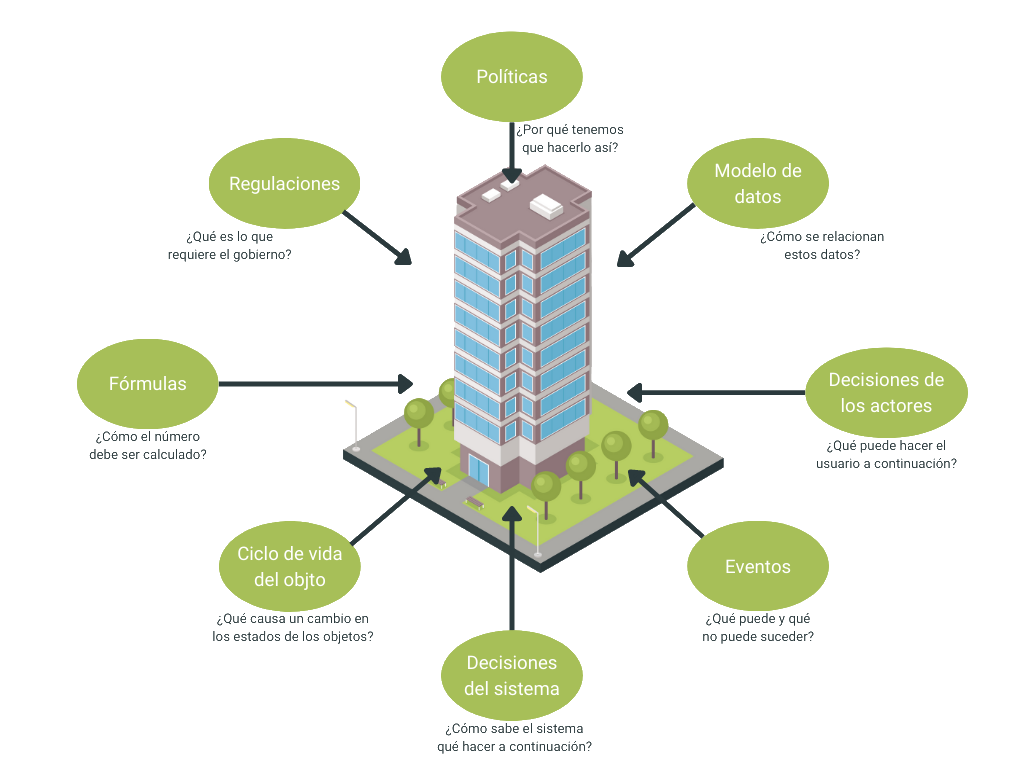
\includegraphics[width=0.9\textwidth]{imgs/9.png}
        \end{figure}
        
        \newpage
        
        \textbf{Documento SRS}
        
        Un SRS es un documento cuyo propósito es proporcionar una descripción completa de un producto de software a desarrollar, incluyendo su propósito, los principales procesos de negocio que serán soportados, características, parámetros clave de rendimiento y comportamiento.
        
        Estructura del documento:
        
        \begin{figure}[h]
            \centering
            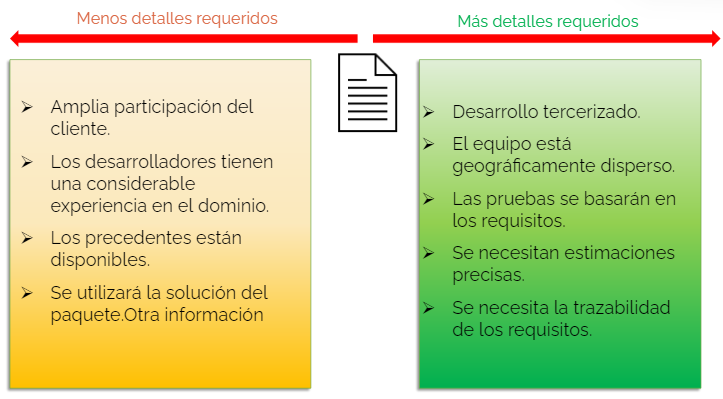
\includegraphics[width=0.7\textwidth]{imgs/10.png}
        \end{figure}
    
        ¿Cuánto tiempo es necesario invertir en ello?
        
        \begin{figure}[h]
            \centering
            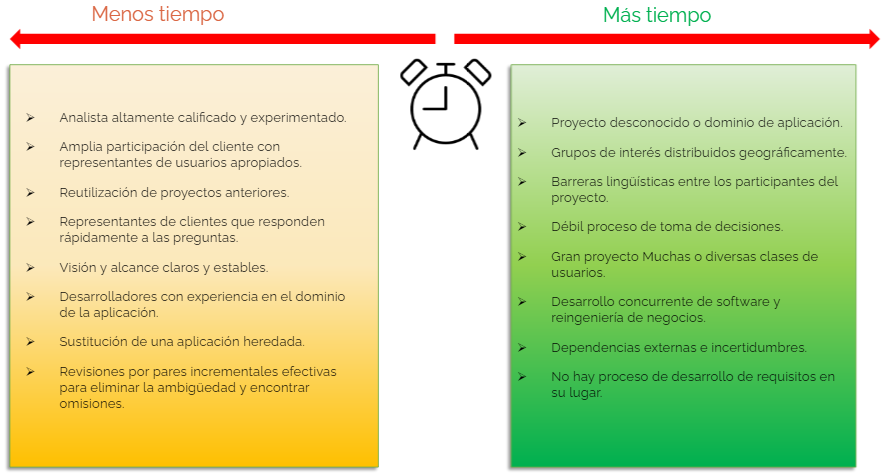
\includegraphics[width=0.7\textwidth]{imgs/11.png}
        \end{figure}
        
        \newpage
        
        \textbf{Planguage}
        
        Planguage consiste en un lenguaje de especificación y un set correspondiente de descripción de métodos o procesos para la especificación, el análisis, el diseño y la gestión de procesos en proyectos u organizaciones.
        
        Ejemplo:
        
        \begin{multicols}{2}
            \begin{itemize}
            \item \textbf{Requerimientos no funcionales} (Versión 1): 
            "El sistema debe ser fácil de aprender"
            \item \textbf{Requerimientos no funcionales} (Versión 2): 
            "El sistema debe ser usado exitosamente para crear una orden de trabajo en menos de 10 minutos sin ningún tipo de ayuda por lo menos para el 80\% del personal sin ningún tipo de experiencia en el uso del sistema"
            
            \item[]
            
            \item[]
            
            \item[]
        \end{itemize}
        
        \begin{Figure}
            \centering
            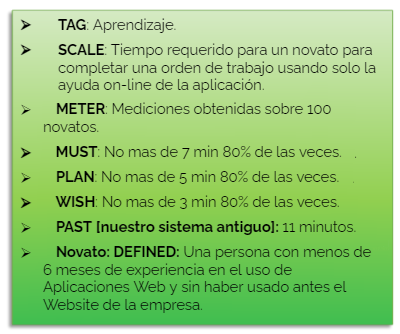
\includegraphics[width=\linewidth]{imgs/12.png}

        \end{Figure}
        \end{multicols}
    
    \subsubsection*{Gestión de requerimientos}
    \addcontentsline{toc}{subsubsection}{Gestión de requerimientos}
    
    \textbf{Actividades centrales de gestión de requisitos:}
    
    \begin{enumerate}
        \item Control de versiones
        \begin{itemize}
            \item Definición de un esquema de identificación de versión
            \item Seguimiento individual de requisitos
            \item Seguimiento de conjunto de requisitos
        \end{itemize}
        \item Control de cambio
        \begin{itemize}
            \item Proponiendo cambios
            \item Análisis de impacto
            \item Tomando decisiones
            \item Actualizar requisitos individuales
            \item Actualización de planes
            \item Medición de la volatilidad de los requisitos
        \end{itemize}
        \item Tracking de estado de requerimientos
        \begin{itemize}
            \item Definición de posibles estados de requisitos
            \item Registrar el estado de cada requisito
            \item Seguimiento de la distribución del estado de todos los requisitos
        \end{itemize}
        \item Trazado de requerimientos
        \begin{itemize}
            \item Definición de enlaces a otros requisitos
            \item Definir enlaces a otros elementos del sistema
        \end{itemize}
    \end{enumerate}
    
    \newpage
    
    \textbf{Pautas para gestión de requisitos}\\
    
    \textbf{Control de versiones:}\\
    
    Cada requisito debe incorporar:
    
    \begin{itemize}
        \item Fecha de creación del requisito
        \item Número de versión actual del requisito
        \item Autor que escribió el requisito
        \item Prioridad
        \item Estado
        \item Origen o fuente del requisito
        \item Justificación del requisito
        \item Número de versión o iteración a la que se asigna el requisito
        \item Partes interesadas para contactar con preguntas o tomar decisiones sobre los campos propuestos
        \item Método de validación a utilizar o criterios de aceptación
    \end{itemize}
    
    \textbf{Control de cambios:}
    
    Modelo para el control de cambio:
    
    \begin{enumerate}
        \item Propósito y alcance
        \item Roles y responsabilidades
        \item Cambio de estados de solicitudes
        \item Criterios de entrada
        \item Tareas
            \begin{enumerate}
                \item[5.1] Evaluar la solicitud de cambio
                \item[5.2] Decidir sobre el cambio
                \item[5.3] Implementar el cambio
                \item[5.4] Verificar el cambio
            \end{enumerate}
        \item Criterios de salida
        \item Informes de estado del control de cambio
        \item[] Anexos: Atributos guardados para cada solicitud
        
    \end{enumerate}
    
    Preguntas para entender las posibles implicancias del cambio propuesto:
    
    \begin{itemize}
        \item 
    \end{itemize}
    
    \subsubsection*{Elicitación}
    \addcontentsline{toc}{subsubsection}{Elicitación}
    
    
    
    \subsubsection*{Análisis}
    \addcontentsline{toc}{subsubsection}{Análisis}
    
%    \subsection*{Las historias de usuario}
    \addcontentsline{toc}{subsection}{Las historias de usuario}
    
    \subsubsection*{¿En qué parte del proceso de desarrollo aparece el testing?}     
    \addcontentsline{toc}{subsubsection}{¿En qué parte del proceso de desarrollo aparece el testing?}
    
    El modelo definido para para este tipo de proyectos de desarrollo de software usa \textit{como base} un enfoque simplificado de \textbf{UP} (Unified Process), denominado OpenUp. Sus principales características son:
    
    \begin{itemize}
        \item Aplica el enfoque incremental e iterativo
        \item Filosofía ágil centrada en la colaboración en proyectos de software
        \item Un proceso liviano
        \item Independiente de las herramientas
        \item Puede ser lo suficientemente formal para llevar a cabo los presentes desarrollos
    \end{itemize}
    
    Este posee cuatro fases, listadas a continuación:
    
    \begin{enumerate}
        \item \textbf{Iniciación}
        
            Se trata de comprender el alcance y objetivos e información para decidir si continuar o no con el proyecto. Se basa en comprender lo que se va a construir, identificar sus funcionalidades clave, determinar una posible solución y comprender a alto nivel costos, riesgos y alcances.
            
        \item \textbf{Elaboración}
        
            Detalla los requerimientos del software. Diseña, valida y establece una línea base para el desarrollo. Mitiga los riesgos más importantes, aquí se definen la programación y la estimación de los gastos.
            
        \item \textbf{Construcción}
        
            Se centra en el diseño, implementación y pruebas de las funciones a desarrollar. Se basa en las definiciones de la línea base. Se desarrolla iterativamente el producto, se cierran eventuales nuevos requisitos y pruebas. Aquí se busca minimizar los costos en desarrollo, obtener sinergia en el equipo y lograr paralelismo.
            
        \item \textbf{Transición}
        
            La finalidad de esta fase es asegurar que el software esté listo para la entrega a los usuarios. Se realizan ajustes finos (en rendimiento y calidad del producto de la fase anterior). Se realizan pruebas para validar que las expectativas de los usuarios se cumplen, esto puede implicar varios niveles de pruebas de aceptación del producto, incluidas las pruebas formales e informales. Se espera que se pueda entregar el producto, además de mejorar el desempeño en futuros proyectos a través de lecciones aprendidas en el actual. Estas lecciones deben ser documentadas, para así mejorar el proceso, el entorno y las herramientas.
            
    \end{enumerate}
    
    \begin{figure}[h]
        \begin{multicols}{2}
            \centering
            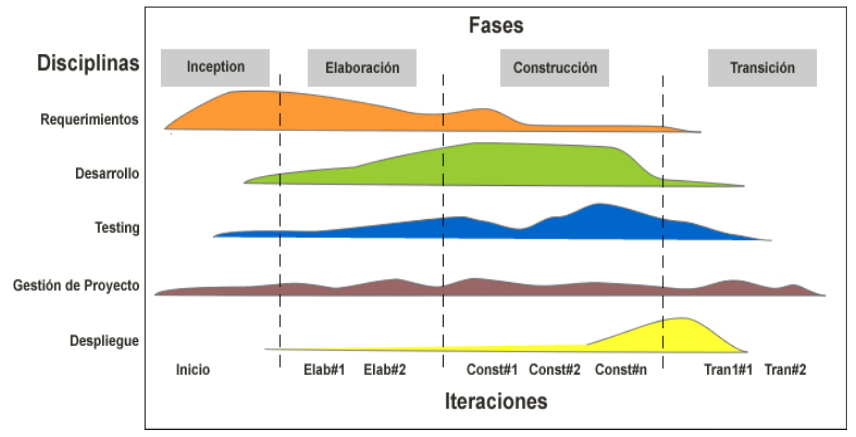
\includegraphics[width=0.48\textwidth]{imgs/5.png}
            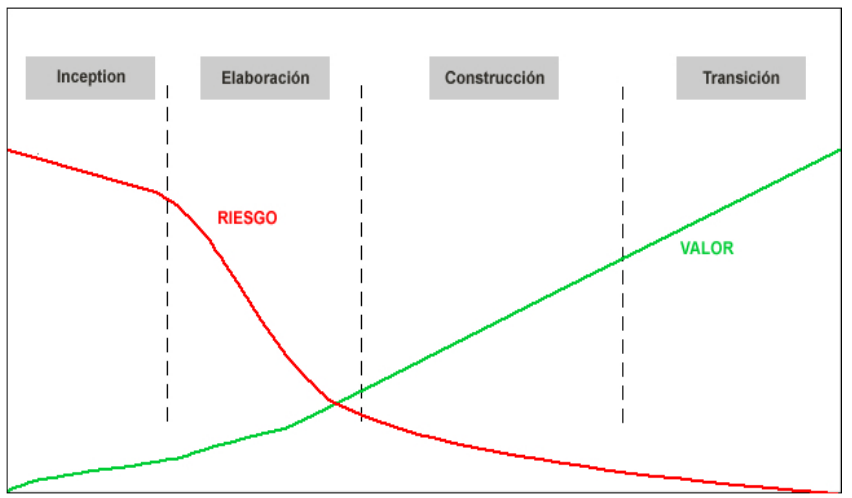
\includegraphics[width=0.42\textwidth]{imgs/6.png}
        \end{multicols}
    \end{figure}